% *********************************************************************
% © 2021-2023 Jeremy Sylvestre
%
% Permission is granted to copy, distribute and/or modify this document
% under the terms of the GNU Free Documentation License, Version 1.3 or
% any later version published by the Free Software Foundation; with no
% Invariant Sections, no Front-Cover Texts, and no Back-Cover Texts. A
% copy of the license is included in the appendix entitled “GNU Free
% Documentation License” that appears in the output document of this
% PreTeXt source code. All trademarks™ are the registered® marks of
% their respective owners.
%
% *********************************************************************

\newcommand*{\xmin}{0}
\newcommand*{\xmax}{10}
\newcommand*{\shortxmax}{9.95}
\newcommand*{\ymin}{0}
\newcommand*{\ymax}{6}

%
% DE is y' = r (y - T) y
%
% We are using r = 1 and T = 4
%
% Solutions curves are
%   y = 4 / (1 - A e^{4t})
% where
%   A = (y0 - 4) / y0
% BUT
% solutions are h.scaled by factor of 10

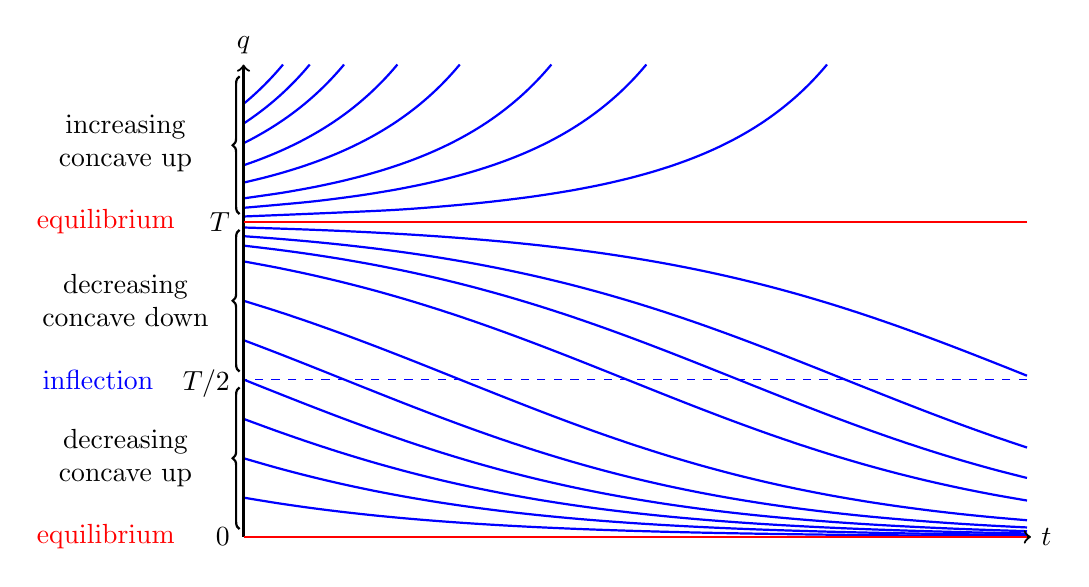
\begin{tikzpicture}
[
	closedpt/.style={circle,draw,fill,inner sep=0pt,minimum size=4pt},
	openpt/.style={circle,draw,inner sep=0pt,minimum size=4pt}
]

	\draw[dashed,blue] (\shortxmax,2) -- (\xmin,2);
	\node[left,xshift=-0.05cm,yshift=-0.05cm] at (0,2) {$T/2$};
	\node[blue,xshift=-1.5cm] at (-0.35,2) {inflection};

	\draw[thick, decorate, decoration = {brace}, xshift=-0.05cm] (0,4.1) -- (0,5.85);
	\node[align=center,xshift=-1.5cm] at (0,5) {increasing \\ concave up};

	\draw[thick, decorate, decoration = {brace}, xshift=-0.05cm] (0,2.1) -- (0,3.9);
	\node[align=center,xshift=-1.5cm] at (0,3) {decreasing \\ concave down};

	\draw[thick, decorate, decoration = {brace}, xshift=-0.05cm] (0,0.1) -- (0,1.9);
	\node[align=center,xshift=-1.5cm] at (0,1) {decreasing \\ concave up};

	\foreach \q in {0.5,1,1.5,2,2.5,3,3.5,3.7,3.82,3.93} {
		\draw[thick,blue,smooth,domain=0:\shortxmax] plot (\x, { 4 / (1 + (4 - \q) * exp(4*\x / 10) / \q) });
	}

	% above q = T = 4, things become exponential
	% so invert to t = ...
	% so that we can control range instead of domain
	\foreach \q in {4.07,4.18,4.3,4.5,4.72,5,5.25,5.5} {
		\draw[thick,blue,smooth,domain=\q:\ymax] plot ({ 10 * (ln( \q * (4 - \x) / (\x * (4 - \q)) )) / 4 }, \x);
	}

	% axes
	\draw[->,thick] (\xmin,0) -- (\xmax,0) node[right] {$t$};
	\draw[->,thick] (0,\ymin) -- (0,\ymax) node[above] {$q$};

	\foreach \q in {0,4} {
		\draw[red,thick] (\shortxmax,\q) -- (\xmin,\q);
		\node[red,xshift=-1.75cm] at (0,\q) {equilibrium};
	}
	\node[left,xshift=-0.05cm] at (0,0) {$0$};
	\node[left,xshift=-0.05cm] at (0,4) {$T$};

\end{tikzpicture}
